%%%%%%%%%%%%%%%%%%%%%%%%%%%%%%%%%%%%%%%%%%%%%%%%%%%%%%%%%%%%%%%%%%%%%%%%%%%%%%%%%%%%%%%%%%%%%%%%%%%
%%%%%%%%%%%%%%%%%%%%%%%%%%%%%%%%%%%%%%%%%%%%%%%%%%%%%%%%%%%%%%%%%%%%%%%%%%%%%%%%%%%%%%%%%%%%%%%%%%%
%%%%%%%%%%%%%%%%%%%%%%%%%%%%%%%%%%%%%%%%%%%%%%%%%%%%%%%%%%%%%%%%%%%%%%%%%%%%%%%%%%%%%%%%%%%%%%%%%%%
%%%%%%%%%%%%%%%%%%%%%%%%%%%%%%%%%%%%%%%%%%%%%%%%%%%%%%%%%%%%%%%%%%%%%%%%%%%%%%%%%%%%%%%%%%%%%%%%%%%

\section{Conceptos}

La exposición se divide en dos subsecciones marcadamente diferentes: fisiología/psicología y 
matemáticas.
En la primera se menciona al deterioro cognitivo en adultos mayores, con énfasis en su 
caracterización dentro del sistema nervioso.
La segunda subsección se centra en las herramientas estadísticas utilizadas para analizar datos 
experimentales, entendidas no como simples \textit{técnicas} sino como objetos abstractos
definidos formalmente.

Estas dos partes difieren no sólo en temas sino también epistemológicamente: en la
primera aparecen afirmaciones basadas en datos experimentales, acompañadas de las citas 
pertinentes, mientras que en la segunda las
afirmaciones son formalmente verdaderas y demostrables en el sistema 
axiomático usual. Respecto a estas últimas, varias de las demostraciones se presentan como 
apéndice junto las definiciones pertinentes, mientras otras son citadas debido a diversos motivos.

\subsection{Psicología}

%La demencia es un síndrome debido a la disfunción cerebral, que produce desintegración
%de la conducta en los planos intelectual y emocional, alterando significativamente la
%función social y laboral del paciente.

La \textbf{demencia} es, según el Manual diagnóstico de y estadístico de trastornos mentales
(DSM-IV), un síndrome que consiste en el desarrollo de déficit cognoscitivos
suficientemente graves como para interferir significativamente en las actividades laborales 
y sociales, respecto al nivel de actividad previo. Aparece precedida por una enfermedad médica o
el efecto de exposición prolongada a sustancias tóxicas, incluso ambos.
Los sujetos con demencia tienen una baja capacidad para aprender información nueva y 
suelen olvidar lo aprendido anteriormente, siendo éste el síntoma más prominente \cite{DCM_5}.

En lo siguiente se considera el 
\textbf{deterioro cognitivo leve}, etapa precusora a la demencia definida como
síndrome caracterizado por una alteración adquirida y prolongada de una o varias funciones 
cognitivas, que no corresponde a un síndrome focal y no cumple criterios suficientes de 
gravedad para ser calificada como demencia \cite{Robles02}.
En el transcurso de este escrito este padecimeinto
será manejado como \textbf{posible deterioro cognitivo (PDC)} ya
que el autor no tiene la autoridad ni la autorización para otorgar un diagnóstico clínico, y porque
los síntomas en esta etapa son --afortunadamente-- reversibles.

Cuando un sujeto presenta cambios marcados en su conducta, es relativamente fácil identificar
la demencia; caso contrario es el diagnóstico temprano de la misma, el cual es importante
para un tratamiento adecuado que 
revierta o desacelere el avance de este síndrome.
Se ha señalado que los criterios del manual DSM-IV son suficientes para este diagnóstico
\cite{Knopman01}.

Al momento de diagnosticar deterioro cognitivo, deben tenerse en cuenta
el envejecimiento normal y la \textbf{pseudodemencia depresiva}, condiciones
con características clínicas similares. Con respecto a ésta última, se define como un
transtorno del afecto y que produce un aparente deterioro cognitivo;
si bien no constituye efectivamente una demencia, puede desencadenar en ello sin un
tratamiento adecuado.

------

En psicología los instrumentos de medición estándar son las pruebas, entendidas como muestras
de alguna conducta de interés a las que se asignan puntajes para comparar cuantitativamente
entre sujetos \cite{Ardila12}.

Las habilidades medibles a través de test neuropsicológicas se suelen agrupar en áreas o
\textbf{dominios}: atención, lenguaje, cálculo, memoria y aprendizaje, percepción,
motricidad, funciones somatosensoriales, habilidades espaciales, funciones ejecutivas. 
%Principales sindromes neuropsicologicos
%Afasia 
%Alexia 
%Agrafia 
%Acalculia 
%Agnosia 
%Apraxia 
%Amnesia 
%Sindrome disejecutivo 
%Demencia
%No  existe  un  manual  de  síndromes  neuropsicológicos,  aunque  muchos  de  ellos  se incluyen 
%en el Manual Diagnóstico y Estadístico de los Trastornos Mentales (DSM-IV, 1994)  y  en  la 
%Clasificación  Internacional  de  las  Enfermedades (ICD-10,  World  Health Organization, 2007).

HACER, QUIZA, UN CUADRO SOBRE LOS DOMINIOS Y SUS RELACIONES CON LAS PARTES DEL CEREBRO

\subsection{Fisiología}

\begin{figure}
\centering
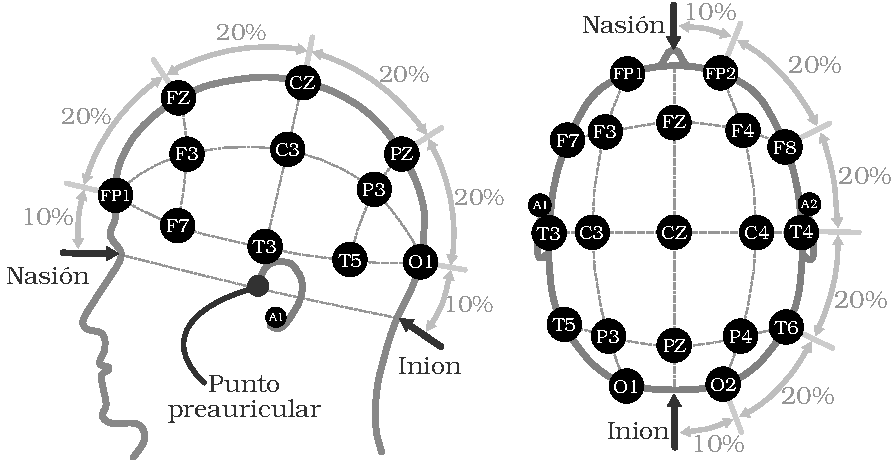
\includegraphics[width=\linewidth]{./img_diagramas/cabeza_proporcionada.pdf} 
\caption{Colocaci\'on de electrodos seg\'un el sistema 10--20. En el cr\'aneo, el \textbf{inion} es 
una protuberancia craneal, mientras que el \textbf{nasi\'on} es la uni\'on del hueso frontal y los 
huesos nasales; el \textbf{punto preauricular} se ubica arriba del cart\'ilago llamado tragus, que 
protege el canal auditivo \cite{Butkov07}. 
}
\label{img1020}
\end{figure}



\subsection{Sueño}

%textwidth: \printinunitsof{cm}\prntlen{\textwidth}
%
%linewidth: \printinunitsof{cm}\prntlen{\linewidth}

%%%%%%%%%%%%%%%%%%%%%%%%%%%%%%%%%%%%%%%%%%%%%%%%%%%%%%%%%%%%%%%%%%%%%%%%%%%%%%%%%%%%%%%%%%%%%%%%%%%
%%%%%%%%%%%%%%%%%%%%%%%%%%%%%%%%%%%%%%%%%%%%%%%%%%%%%%%%%%%%%%%%%%%%%%%%%%%%%%%%%%%%%%%%%%%%%%%%%%%
%%%%%%%%%%%%%%%%%%%%%%%%%%%%%%%%%%%%%%%%%%%%%%%%%%%%%%%%%%%%%%%%%%%%%%%%%%%%%%%%%%%%%%%%%%%%%%%%%%%
%%%%%%%%%%%%%%%%%%%%%%%%%%%%%%%%%%%%%%%%%%%%%%%%%%%%%%%%%%%%%%%%%%%%%%%%%%%%%%%%%%%%%%%%%%%%%%%%%%%
